\documentclass[12pt, a4paper]{article}

\usepackage[czech]{babel}
\usepackage{lmodern}
\usepackage[utf8]{inputenc}
\usepackage[T1]{fontenc}
\usepackage{graphicx}
\usepackage{amsmath}
\usepackage[hidelinks,unicode]{hyperref}
\usepackage{float}
\usepackage{listings}
\usepackage{tikz}
\usepackage[final]{pdfpages}
\usetikzlibrary{shapes,positioning,matrix,arrows}

\newcommand{\img}[1]{(viz obr. \ref{#1})}

\lstset{basicstyle=\ttfamily,
showstringspaces=false,
commentstyle=\color{red},
keywordstyle=\color{blue}
}


\begin{document}
    \begin{titlepage}

        \centering

        \vspace*{\baselineskip}

        \begin{figure}[H]
            \centering
            
\includegraphics[width=7cm]{fav-logo.png}
        \end{figure}

        \vspace*{1\baselineskip}
        {\sc Semestrální práce z předmětu KIV/UPS}
        \vspace*{1\baselineskip}

        \vspace{0.75\baselineskip}

        {\LARGE\sc Realtime online multiplayer hra - Asteroidy \\}

        \vspace{4\baselineskip}

        {\sc\Large Patrik Janoušek \\}

        \vspace{0.5\baselineskip}

        {A17B0231P}\\
        {janopa@students.zcu.cz}

        \vfill

        {\sc Západočeská univerzita v Plzni\\
        Fakulta aplikovaných věd}


    \end{titlepage}


    \tableofcontents
    \pagebreak

    \newpage

    \section{Popis hry}
    Vypracovaná hra Asteroidy je velmi inspirována originální hrou Asteroids z roku 1979.
    Avšak je převzata spíše původní myšlenka hry, na kterou jsou aplikovány vlastní nápady a úpravy.

    Jedná se o hru s velmi primitivními pravidly.
    Hráč ovládá vesmírnout loď, se kterou má možnost střílet do okolních asteroidů nebo hráčů.
    Zároveň může umřít za předpokladu, že ho sestřelí jiný hráč, nebo se středne s letícím asteroidem.
    V takovém případě je hráč přesunut na jinou pozici a je mu udělena třísekundová imunita.
    Po dobu trvání této imunity je mu samozřejmě znemožněno střílet, aby nebyl zvýhodněn nad ostatními hráči.
    Za smrt se neuděluje žádná penalizace.
    Za zabití protihráče je 1 000 bodů, za asteroid je to pak 1-100 bodů podle jeho velikosti.
    Hra končí ve chvíli, kdy nějaký hráč dosáhne 10 000 bodů.

    \begin{figure}[H]
        \makebox[\textwidth]{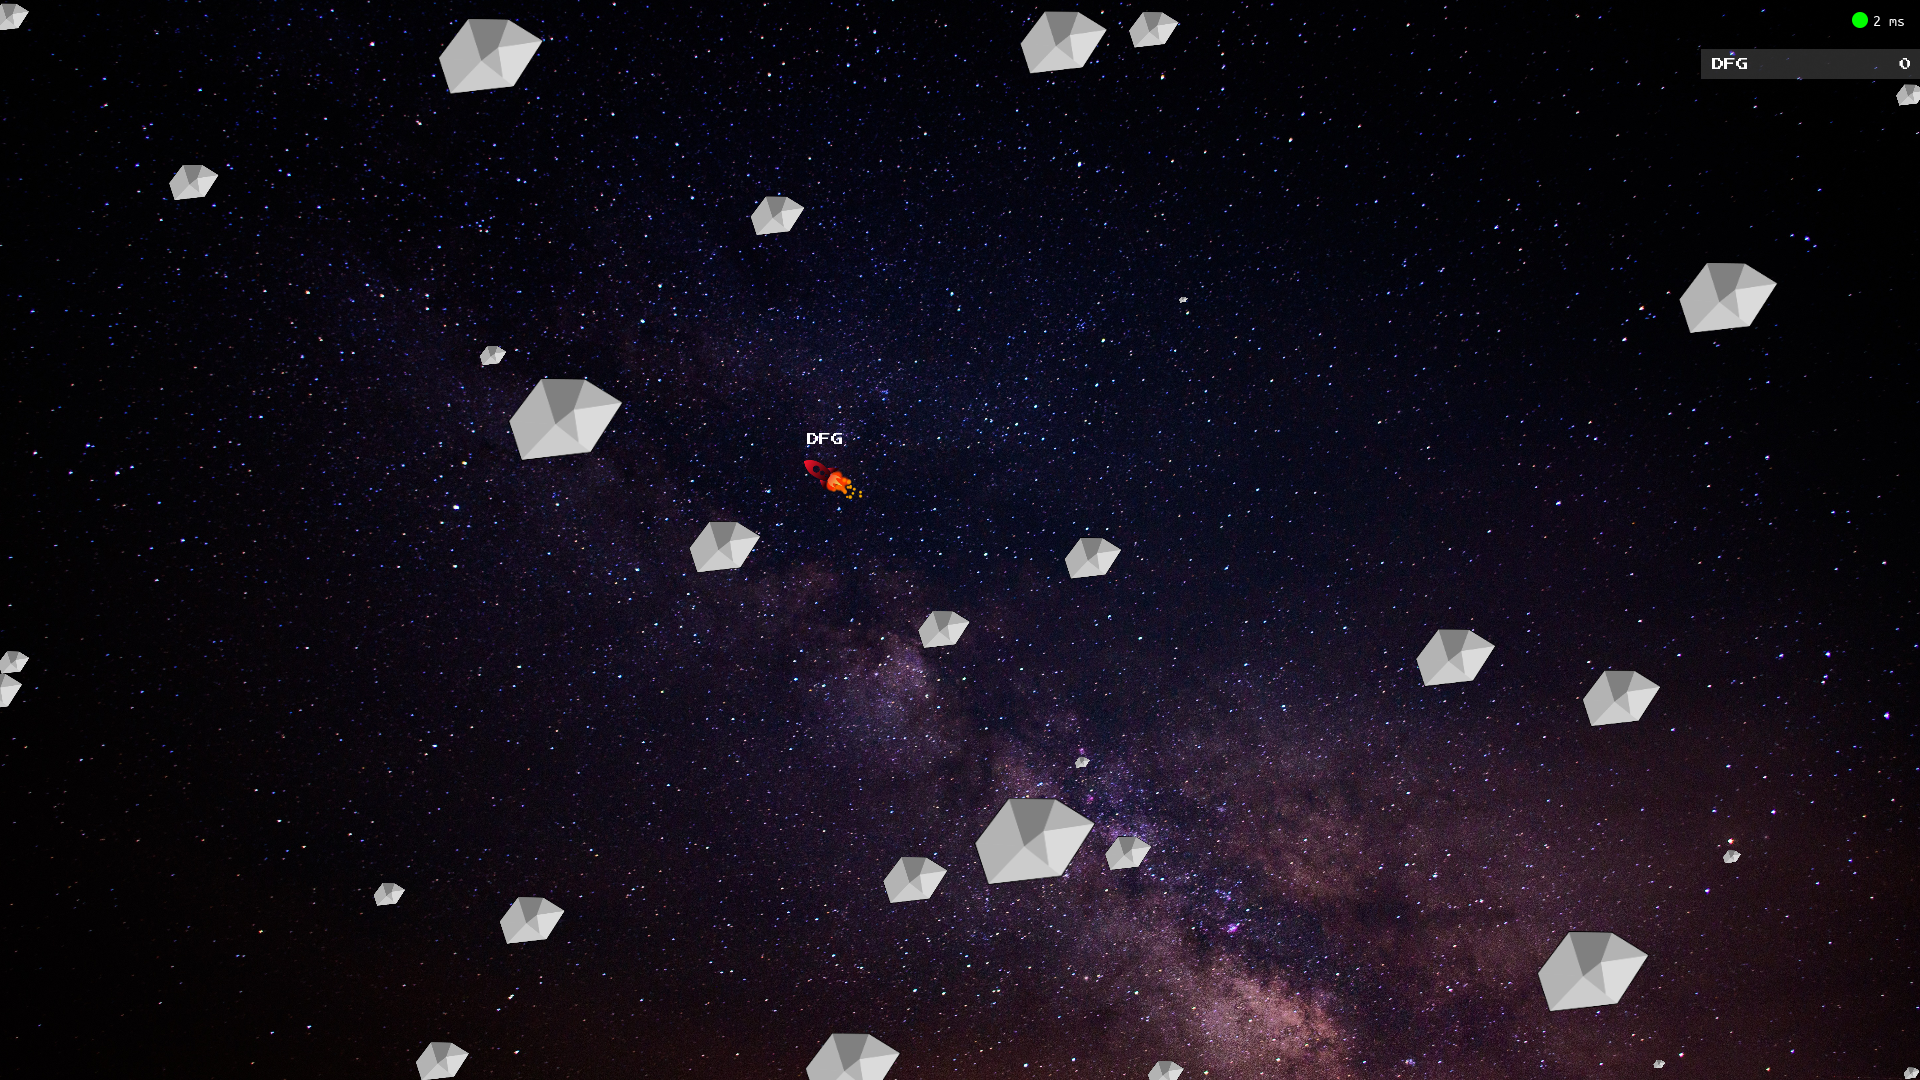
\includegraphics[width=\textwidth]{game}}
        \caption{Snímek z vypracované hry asteroidy}
    \end{figure}

    \section{Protokol}
    \subsection{Specifikace}
    Protokol byl navržen s ohledem na jednoduchost implementace, ale aby zároveň splnil všechny požadavky, které by aplikace mohla mít.
    
    Mezi hlavní požadavky na protokol byla identifikace typu zprávy.
    Tu je možné provádět pomocí trojciferných číselných identifikátorů.
    Díky těmto identifikátorů je schopná komunikující protistrana předpokládat strukturu příchozích dat.

    Podporuje tedy identifikaci zpráv, kde si klient může určit vlastní identifikátor zprávy, a server tento identifikátor zapíše i do odpovědi, díky čemuž je klient schopen poznat na jakou zprávu server odpovídá.
    Tento identifikátor má variabilní délku, tudíž je zde i možnost jeho nepoužití.

    Tělo zprávy je pak zakódované ve formátu JSON, kde je pro klíče použita konvence snake case. 

    \begin{table}[H]
        \centering
        \begin{tabular}{|l|c|c|}
            \hline
            Popis & Délka & Hodnota\\
            \hline
            \hline
            Dělící znak & 1 & \uv{|} \\
            \hline
            Typ zprávy & 3 & Číslo v ASCII \\
            \hline
            Dělící znak & 1 & \uv{|} \\
            \hline
            Délka těla zprávy & variabilní & Číslo v ASCII \\
            \hline
            Dělící znak & 1 & \uv{|} \\
            \hline
            Identifikátor požadavku & variabilní & Řetězec znaků a-z, A-Z a 0-9 v ASCII \\
            \hline
            Dělící znak & 1 & \uv{|} \\
            \hline
            Tělo zprávy & variabilní & Data zakódovaná v JSONu \\
            \hline
        \end{tabular}
        \caption{Specifikace protokolu}
    \end{table}

    \section{Implementace}
    \subsection{Popis hry}

    \subsection{Definice použitých zpráv}
    Jak již bylo uvedeno výše, každý typ zprávy má svůj unikátní trojciferný identifikátor.
    Tento identifikátor může být z hlediska protokolu libovolný, nicméně pro lepší orientaci byla v konkrétní implementaci vytvořena určitá pravidla.
    
    A to taková, že identifikátor 1xx je použit pro obecné zprávy, které nemusí přímo souviset se samotnou aplikací (keep-alive, atd\dots).
    2xx pak slouží pro zprávy zasílané klientem, a 3xx zprávy zasínalé serverem.
    Zde je ještě dodržováno to, že \uv{xx} je stejné pro klientskou i serverovou zprávu, pokud je serverová zpráva odpovědí na klientský požadavek.
    Tyto identifikátory jsou použity pro zprávy, které přímo nesouvisí se hrou, ale spíše s její správou (autentizace, založení lobby, získání seznamu hráčů, \dots).
    Nakonec jsou pak použity identifikátory zpráv 4xx a 5xx, kde 4xx jsou zprávy zasílané klientem, a 5xx zprávy zasílané serverem. Tyto identifikátory jsou použity pro zprávy přímo související se hrou (pohyb hráče po herní ploše, střelba, \dots).

    Všechny zprávy zasílané serverem, jsou obalovány do struktury, která umožňuje k zasílaným datům přidat status, a případně nějakou dodatečnou zprávu. Přenášená zpráva je pak dostupná pod klíčem \uv{data}.

    \begin{table}[H]
        \centering
        \begin{tabular}{|l|c|}
            \hline
            Klíč & Datový typ\\
            \hline
            \hline
            data & object \\
            \hline
            message & string \\
            \hline
            status & boolean \\
            \hline
        \end{tabular}
        \caption{Obalovací zpráva serveru}
    \end{table}

    \subsubsection{Zprávy zasílané klientem}
    \subsubsection*{KeepAlive}
    Typ zprávy: 100\\

    Tato zpráva je zasílána klientem, aby ověřila funkčnost spojení se serverem, a zároveň schopnost komunikace mezi těmito dvěmi stranamy.

    \begin{table}[H]
        \centering
        \begin{tabular}{|l|c|}
            \hline
            Klíč & Datový typ\\
            \hline
            \hline
            ping & string \\
            \hline
        \end{tabular}
        \caption{Specifikace KeepAlive}
    \end{table}

    Klient jako hodnotu pole \uv{ping} vyplňuje řetězec \uv{pong}. A server na tuto zprávu odpovídá stejným typem zprávy, jen jako hodnotu pole \uv{ping} vyplňuje řetězec \uv{ping-pong}.

    \subsubsection*{ActionError}
    Typ zprávy: 101\\

    Zpráva, která je zasílána serverem jako odpověď na typ zprávy, ke které klient nemá oprávnění, nebo daná zpráva neexistuje.
    Tato zprávy má prázdné tělo a neposílá žádná dodatečná data.

    \subsubsection*{Authenticate}
    Typ zprávy: 200\\

    Autentizační zpráva musí být klientem zaslána jako první zpráva po připojení k serveru.
    V případě neposlání této zprávy nemá klient žádné pravomoce, mimo zasílání \textit{KeepAlive}.

    \begin{table}[H]
        \centering
        \begin{tabular}{|l|c|c|}
            \hline
            Klíč & Datový typ & Popis\\
            \hline
            \hline
            name & string & Jméno hráče\\
            \hline
        \end{tabular}
        \caption{Specifikace Authenticate}
    \end{table}

    \subsubsection*{CreateLobby}
    Typ zprávy: 201\\

    Zpráva určená k založení lobby.
    Hráč, který lobby vytváří, je automaticky do lobby připojen a není již potřeba posílat \textit{JoinLobby}.

    \begin{table}[H]
        \centering
        \begin{tabular}{|l|c|c|}
            \hline
            Klíč & Datový typ & Popis\\
            \hline
            \hline
            name & string & Název lobby\\
            \hline
            players\_limit & integer & Limit počtu hráčů v lobby\\
            \hline
        \end{tabular}
        \caption{Specifikace Authenticate}
    \end{table}

    \subsubsection*{DeleteLobby}
    Typ zprávy: 202\\

    Zpráva určená ke smazání lobby.
    Ačkoliv zpráva přjímá jako parametr název lobby ke smazání, tak hráč má právo smazat lobby jenom za předpokladu, že je jejím vlastníkem.

    \begin{table}[H]
        \centering
        \begin{tabular}{|l|c|c|}
            \hline
            Klíč & Datový typ & Popis\\
            \hline
            \hline
            name & string & Název lobby ke smazání\\
            \hline
        \end{tabular}
        \caption{Specifikace DeleteLobby}
    \end{table}

    \subsubsection*{ListLobbies}
    Typ zprávy: 203\\

    Prázdná zpráva sloužící k získání seznamu všech dostupných lobby.

    \subsubsection*{JoinLobby}
    Typ zprávy: 204\\

    Zpráva sloužící k připojení do lobby.
    Připojení je možné pouze za předpokladu, že je v lobby volný slot pro hráče.
    Tato skutečnost je ověřována serverem, který vyplní patřičný status zprávy.

    \begin{table}[H]
        \centering
        \begin{tabular}{|l|c|c|}
            \hline
            Klíč & Datový typ & Popis\\
            \hline
            \hline
            name & string & Název lobby k připojení\\
            \hline
        \end{tabular}
        \caption{Specifikace JoinLobby}
    \end{table} 

    \subsubsection*{LeaveLobby}
    Typ zprávy: 214\\

    Prázdná zpráva, kterou se hráč odpojí z lobby.

    \subsubsection*{ListLobbyPlayers}
    Typ zprávy: 206\\

    Prázdná zpráva sloužící k získání seznamu hráčů přípojených do lobby.

    \subsubsection*{StartGame}
    Typ zprávy: 207\\\\
    Prázdná zpráva pro spuštění hry.
    Tuto zprávu může poslat libovolný hráč z lobby.
    Od této chvíle je na serveru vytvořená instance hry, a všichni hráči jsou neustále informováni o jejím stavu.

    \subsubsection*{GameReconnectAvailable}
    Typ zprávy: 211\\

    Touto prázdnou zprávou si může klient ověřit, zda připojený hráč nepatří do nějaké hry, a tudíž se do ní může opět připojit, nebo se z ní odpojit.

    \subsubsection*{Reconnect}
    Typ zprávy: 212\\

    Zasláním této prázdné zprávy se hráč připojí zpět do probíhající hry, kterou předtím opustil.

    \subsubsection*{LeaveGame}
    Typ zprávy: 213\\

    Zasláním této prázdné zprávy hráč definitivně opustí probíhající hru, ze které odešel, a již se do ní nemůže vrátit.
   
    \subsubsection*{PlayerMove}
    Typ zprávy: 400\\

    Zpráva, která informuje server o změně atributů hráče.
    Tuto zprávu by měl klient posílat při změně své pozice, nebo libovolného atributu svého pohybu (vektor pohybu, rotace, \dots).
    Zaslané údaje jsou na serveru verifikovány a v případě chybně zaslaných údajů je klient vyžádán k synchronizaci údajů se serverem (viz. \textit{UpdateState}).

    \begin{table}[H]
        \centering
        \begin{tabular}{|l|c|c|}
            \hline
            Klíč & Datový typ & Popis\\
            \hline
            \hline
            pos\_x & double & Pozice na ose X\\
            \hline
            pos\_y & double & Pozice na ose Y\\
            \hline
            velocity\_x & double & Složka X vektoru pohybu\\
            \hline
            velocity\_y & double & Složka Y vektoru pohybu\\
            \hline
            rotation & double & Rotace hráče v radiánech\\
            \hline
        \end{tabular}
        \caption{Specifikace PlayerMove}
    \end{table}

    \subsubsection*{ShootProjectile}
    Typ zprávy: 401\\

    Prázdná zpráva informující server o vystřelení projektilu

    \subsubsection{Zprávy zasílané serverem}
    \subsubsection*{CreatedLobbyResponse}
    Typ zprávy: 301\\
    Odpověď na zprávu: \textit{CreatedLobbyResponse}\\

    Prázdná zpráva, kterou je klient informován o založení lobby.

    \subsubsection*{DeleteLobbyResponse}
    Typ zprávy: 302\\

    Prázdná zpráva, kterou je klient informován o smazání lobby.

    \subsubsection*{ListLobbiesResponse}
    Typ zprávy: 303\\
    Odpověď na zprávu: \textit{ListLobbies}\\

    Tuto zprávu server používá pro zaslání seznamu všech dostupných lobby.
    V kořenu zprávy je jedinný klíč \uv{lobbies}, který má následující strukturu:

    \begin{table}[H]
        \centering
        \begin{tabular}{|l|c|c|}
            \hline
            Klíč & Datový typ & Popis\\
            \hline
            \hline
            name & string & Název lobby\\
            \hline
            connected\_players & integer & Počet hráčů připojených do lobby\\
            \hline
            players\_limit & integer & Maximální počet připojených hráčů\\
            \hline
        \end{tabular}
        \caption{Specifikace ListLobbiesResponse}
    \end{table}

    \subsubsection*{JoinLobbyResponse}
    Typ zprávy: 304\\
    Odpověď na zprávu: \textit{JoinLobby}\\

    Prázdná zpráva informující klienta o stavu připojení do lobby.

    \subsubsection*{PlayerLobbyJoined}
    Typ zprávy: 305\\

    Zpráva informující hráče, kteří jsou již připojení v lobby, o připojení nového hráče.

    \begin{table}[H]
        \centering
        \begin{tabular}{|l|c|c|}
            \hline
            Klíč & Datový typ & Popis\\
            \hline
            \hline
            name & string & Jméno hráče\\
            \hline
        \end{tabular}
        \caption{Specifikace ListLobbiesResponse}
    \end{table}

    \subsubsection*{ListLobbyPlayersResponse}
    Typ zprávy: 306\\
    Odpověď na zprávu: \textit{ListLobbyPlayers}\\

    Zpráva, kterou server klientovi vrací seznam hráčů připojených do lobby.

    \begin{table}[H]
        \centering
        \begin{tabular}{|l|c|c|}
            \hline
            Klíč & Datový typ & Popis\\
            \hline
            \hline
            players & string[] & Pole jmen hráčů\\
            \hline
        \end{tabular}
        \caption{Specifikace ListLobbyPlayersResponse}
    \end{table}

    \subsubsection*{StartGameResponse}
    Typ zprávy: 307\\
    Odpověď na zprávu: \textit{StartGame}\\

    Prázdná zpráva, která se zasílá všem hráčům při startu hry.

    \subsubsection*{LobbyPlayerConnected}
    Typ zprávy: 308\\\\
    Zpráva informující ostatní hráče v lobby o připojení nového hráče.

    \begin{table}[H]
        \centering
        \begin{tabular}{|l|c|c|}
            \hline
            Klíč & Datový typ & Popis\\
            \hline
            \hline
            name & string & Jméno příchozího hráče\\
            \hline
        \end{tabular}
        \caption{Specifikace LobbyPlayerConnected}
    \end{table}

    \subsubsection*{LobbyPlayerDisconnected}
    Typ zprávy: 309\\

    Zpráva informující ostatní hráče v lobby o odpojení hráče.

    \begin{table}[H]
        \centering
        \begin{tabular}{|l|c|c|}
            \hline
            Klíč & Datový typ & Popis\\
            \hline
            \hline
            name & string & Jméno odpojeného hráče\\
            \hline
        \end{tabular}
        \caption{Specifikace LobbyPlayerDisconnected}
    \end{table}

    \subsubsection*{GameEnd}
    Typ zprávy: 310\\

    Tato zpráva je zaslána všem hráčům hry po jejím skončení.
    V kořenu zprávy obsahuje jediný klíč \uv{score\_summary}, který obsahuje pole s objekty následující struktury:

    \begin{table}[H]
        \centering
        \begin{tabular}{|l|c|c|}
            \hline
            Klíč & Datový typ & Popis\\
            \hline
            \hline
            player\_name & string & Jméno hráče\\
            \hline
            score & integer & Dosažené skóre\\
            \hline
            winner & boolean & Informaci o tom, zda je daný hráč výherce\\
            \hline
        \end{tabular}
        \caption{Specifikace GameEnd}
    \end{table}

    \subsubsection*{GameReconnectAvailableResponse}
    Typ zprávy: 311\\
    Odpověď na zprávu: GameReconnectAvailable\\

    Zpráva informující o tom, zda je možné se připojit zpět do probíhající hry, ze které se hráč odpojil. Obsahuje pouze jednou hodnotu:

    \begin{table}[H]
        \centering
        \begin{tabular}{|l|c|c|}
            \hline
            Klíč & Datový typ & Popis\\
            \hline
            \hline
            available & boolean & Dostupnost znovupřipojení se do probíhající hry\\
            \hline
        \end{tabular}
        \caption{Specifikace GameReconnectAvailableResponse}
    \end{table}

    \subsubsection*{ReconnectResponse}
    Typ zprávy: 312\\
    Odpověď na zprávu: Reconnect\\

    Prázdná zpráva informující klienta o úspěšném znovupřipojení zpět do hry.


    \subsubsection*{LeaveGameResponse}
    Typ zprávy: 313\\
    Odpověď na zprávu: LeaveGame\\

    Prázdná zpráva informující klienta o úspěšném opuštění probíhající hry.

    \subsubsection*{LeaveLobbyResponse}
    Typ zprávy: 314\\
    Odpověď na zprávu: LeaveLobby\\

    Prázdná zpráva informující klienta o úspěšném opuštění lobby.


    \subsection{Server}
    Pro implementaci serveru byl zvolen jazyk go.
    Jednak z důvodu vyzkoušení nové technologie, ale i z důvodu jeho technologických výhod.
    Zejména z důvodu jednoduchosti paralelizace a možnosti jednoduché a bezpečné komunikace mezi jednotlivými vlákny (resp. gorutinami), ale i automatické správy paměti.

    \subsubsection{Síť}
    Síť je v serveru implementována s důrazem na co největší oddělení od zbytku aplikace, a je vedle aplikace v samostatném balíku \uv{net}, který je pojmenován po vzoru stejnojmenného balíku ze standardní knihovny jazyka go.
    Tento balík obsahuje implementaci jak samotného TCP serveru, tak i protokolu.
    
    Protokol je plně oddělen od TCP serveru, se kterým komunikuje pomocí rour.
    Díky tomu je protokol schopen komunikovat s libovolným binárním streamem dat, který nutně nemusí přijít od TCP serveru.
    Tato vlastnost ho dělá i samostatně testovatelným.
    Nevýhodou však je, že je díky tomu komunikace s protokolem blokující, a každý klient musí mít pro protokol vlastní gorutinu.

    Pokud tedy přijde zpráva, tak jí TCP server přečte ze socketu, a zapíše jí do patřičné roury připojeného klienta, odkud zprávu začne přečte protokol, a zečne jí zpracovávat.
    Po tom, co protokol přečte celou zprávu, tak ji naplní do struktury \texttt{ProtoMessage}, a pomocí kanálu ji předá zpět TCP serveru, který tuto zprávu vezme, přidá k ní odesílatele, a skrz další kanál jí předá master serveru, který může zprávu na základě jejího obsahu a typu dále zpracovávat.

    \subsubsection{Reakce na zprávy}
    Přijatá a dekódovaná správa se pomocí kanálu posílá do takzvaného \textit{master serveru}, který se stará o routing mimoherních zpráv a spouštění akcí s nich svázanými.
    Zároveň se stará o rozesílání výstupů z akcí na tyto požadavky.

    Tyto akce jsou struktury splňující interface \texttt{Action}, díky kterému je možné všechny tyto akce uložit do dvouúrovňového slovníku.
    První úrověň používá jako klíč kontext hráče.
    Tím je už v podstatě návrhem zajištěno, že hráč, který není ve hře, nemůže poslat zprávu o pohybu.
    V druhé úrovni je pak klíčem celočíselný identivikátor zprávy.

    Pokud tedy \textit{master server} přijme zprávu, tak na základě kontextu odesílajícího hráče, a na základě typu zprávy, spustí danou akci.
    Tato akce vrátí \textit{ActionResponse}, který kromě odpovědi dané akce obsahuje také kterým hráčům se má odpověď poslat.
    To z důvodu, aby bylo možné implementovat např. zprávu, která informuje hráče o startu hry.
    Jelikož požadavek posílá pouze jeden hráč, ale informaci o potvrzení startu musí dostat všichni hráčí v lobby.

    \subsubsection{Implementace hry}
    Samotnou hru v aplikaci řeší takzvaný \textit{game server}.
    Tento \textit{game server} je spouštěn pomocí zprávy \textit{StartGame} ve vlastní gorutině.
    Po spuštění dojde k sestavení a inicializaci herního stromu, a nésledné spuštění samotného gameloopu.
    Tento gameloop se pak snaží $30\times$ za sekundu vykonávat herní logiku.
    Implementace gameloopu umí řešit jak nedostatek, tak i přebytek výkonu, kdy se při nedostatku nečeká mezi jednotlivými cykly, čímž se server snaží \uv{dohnat} hru, a naopak při přebytku výkonu se čeká na správný čas, kdy se má provést další logika hry.

    Herní logika je pak implementována tak, že každý uzel herního stromu má funkci \texttt{Process}, který dostává parametr \texttt{delta}, což je čas v sekundách, který uběhl od posledního spuštění, a pak parametr \texttt{playerMessages}, který obsahuje list příchozích zpráv od hráčů.
    Naslouchání na tyto zprávy si může každý node určit pomocí funkce \texttt{ListenMessages}, která umožňuje určit příchozí typy zpráv chce daný node naslouchat.
    Situace, kdy je více instancí jednoho nodu, ale daný hráč může ovládat jen některé, je vyřešená pomocí funkce \texttt{ListenMessages}, kde si daný node může profiltrovat reálné instance příchozích zpráv.

    Přenos stavu hry k hráči je pak řešen zasíláním celého herního stromu.
    Tím se vytváří celkem vysoký datový tok, ale testy ukázaly, že vzhledem k povaze hry je toto řešení použitelné i v reálných podmínkách.

    \subsubsection{Herní objekty}
    V herním stromu jsou uloženy herní objekty typu \texttt{RootNode}, \texttt{Asteroid}, \texttt{Spaceship}, \texttt{Score} a \texttt{Projectile}.

    \subsubsection*{RootNode}
    Tento node je v podstatě prázdný, a slouží jen a pouze jako node, který je v kořenu celého herního stromu, pod který se přidávají další herní objekty.

    \subsubsection*{Asteroid}
    Asteroid je, jak již název hry napovídá, hlavním objektem celé hry.
    Asteroidy můžou mít různou velikost, s čímž souvisí i získané skóre za jeho zničení.
    Krom toho mají ještě svou pozici, vektor rychlosti a rotaci.

    \begin{table}[H]
        \centering
        \begin{tabular}{|l|c|c|}
            \hline
            Klíč & Datový typ & Popis\\
            \hline
            \hline
            pos\_x & double & Pozice asteroidu na ose X\\
            \hline
            pos\_y & double & Pozice asteroidu na ose Y\\
            \hline
            velocity\_x & double & Složka X vektoru pohybu\\
            \hline
            velocity\_y & double & Složka Y vektoru pohybu\\
            \hline
            rotation & double & Rotace asteroidu v radiánech\\
            \hline
            scale & double & Velikost asteroidu\\
            \hline
            value & integer & Získané skóre za zničení asteroidu\\
            \hline
        \end{tabular}
        \caption{Specifikace veřejné části struktury \texttt{Asteroid}}
    \end{table}

    \subsubsection*{Spaceship}
    Tento objekt reprezentuje konkrétní vesmírnou loď hráče, která má možnost střílet ostatní lodě a asteroidy, a také koliduje s asteroidy.
    Kolize s asteroidem způsobí smrt, přesunutí hráče na novou pozici, a udělí mu třísekundovou imunitu.
    Zároveň pokud hráč má imunitu, tak nemůže střílet.

    \begin{table}[H]
        \centering
        \begin{tabular}{|l|c|c|}
            \hline
            Klíč & Datový typ & Popis\\
            \hline
            \hline
            pos\_x & double & Pozice lodi na ose X\\
            \hline
            pos\_y & double & Pozice lodi na ose Y\\
            \hline
            velocity\_x & double & Složka X vektoru pohybu\\
            \hline
            velocity\_y & double & Složka Y vektoru pohybu\\
            \hline
            rotation & double & Rotace lodi v radiánech\\
            \hline
            player\_name & string & Jméno hráče, kterému loď náleží\\
            \hline
            immune & boolean & Indikace, zda má hráč imunitu\\
            \hline
            reload\_position & boolean & Vynucení aktualizace dat na straně klienta\\
            \hline
        \end{tabular}
        \caption{Specifikace veřejné části struktury \texttt{Spaceship}}
    \end{table}

    \subsubsection*{Score}
    \texttt{Score} je objekt, který je zodpovědný za řešení skóre jednotlivých hrářů ve hře.
    Jedná se o poměrně jednoduchý objekt, který s klientem sdílí pouze svou hodnotu, a jméno hráče, kterému náleží.

    \begin{table}[H]
        \centering
        \begin{tabular}{|l|c|c|}
            \hline
            Klíč & Datový typ & Popis\\
            \hline
            \hline
            score & integer & Hodnota skóre\\
            \hline
            player\_name & string & Jméno hráče\\
            \hline
        \end{tabular}
        \caption{Specifikace veřejné části struktury \texttt{Score}}
    \end{table}

    \subsubsection*{Projectile}
    Tento node reprezentuje jednotlivé střely, které hráči vystřelují, a mají velmi podobné atribute, jako ostatní objekty vykreslitelné klientem.

    \begin{table}[H]
        \centering
        \begin{tabular}{|l|c|c|}
            \hline
            Klíč & Datový typ & Popis\\
            \hline
            \hline
            pos\_x & double & Pozice střely na ose X\\
            \hline
            pos\_y & double & Pozice střely na ose Y\\
            \hline
            velocity\_x & double & Složka X vektoru pohybu\\
            \hline
            velocity\_y & double & Složka Y vektoru pohybu\\
            \hline
            rotation & double & Rotace střely v radiánech\\
            \hline
        \end{tabular}
        \caption{Specifikace veřejné části struktury \texttt{Projectile}}
    \end{table}

    \subsubsection{Použité kninhovny}
    Server používá knihovnu logrus na logování.
    Jazyk go sice má logovací knihovnu ve standardní knihovně, nicméně je poměrně strohá a ve spoustě místech nedostačující.
    Logrus nabízí především lepší manipulaci s formátem logu, jeho obarvováním v termináli, a nabízí i mnohem více log levelů.

    Dále byla při vývoji použita knihovna go-spew, která umožňuje vypsání obsahu struktury v rámci všech zanořených strutkur.
    A to i za předpokladu, že jsou v dané struktuře ukazatele.
    Go-spew umí totiž tyto ukazatele automaticky dereferencovat, a vypsat jejich obsah, namísto obsahu ukazatele.

    A nakonec byly využity knihovny yaml a jennifer.
    Yaml, protože v tomto formátu jsou definovány všechny zprávy serveru.
    A knihovna jennifer z důvodu schopnosti generování golang kódu.
    Tato metoda se v go používá jako náhrada chybějící podpory metaprogramování.
    Pomocí jennifer je konfigurační yaml soubor převeden na golang kód ve více souborech, což při vývoji ušetřilo spoustu práce, bez narušení struktury nebo abstrakce kódu.

    \subsection{Klient}
    Klient je implementováín v herním enginu godot.
    Obecně herní engine byl oproti standardním formulářovým frameworkům (Qt, Swing, JavaFX, \dots) z důvodu povahu hry, která je realtime.
    Takováto hra by se dělala ve standardním formulářovém frameworku velmi obtížně.
    Ať už z důvodů technických omezení, tak z důvodu, že formulářové frameworky nejsou vůbec připravené pro tvorbu realtime hry.
    Velká část formulářového frameworku by tak zůstala nevyužita, jelikož by byla potřeba vlastní implementace většiny funkcionalit.

    Konkrétně herní engine godot byl vybrán především z důvodu především dřívější zkušenosti, ale i z důvodu jeho jednoduchosti.
    Zároveň používá vlastní skriptovací jazyk GDScript (resp. GodotScript), který vychází z programovacího jazyka python.
    Nevychází z něj v plné míře. Bohužel chybí spousta věcí, na které jsou python programátoři zvyklí. Nicméně z hlediska syntaxe python velmi připomíná.

    Vzhledem k tomu, že godot aktuálně nemá žádným způsobem vyřešené externí závislosti, a tudíž je používání externích knihoven celkem nepraktické, tak aplikace žádné nepoužívá.

    \subsubsection{Síť}
    Síť je v klientu řešena mnohem jednodušeji než na serveru.
    A to jednak z toho důvodu, že klient komunikuje vždy jen s jednou protistranou, tak i z důvodu, že godot není určen na to, aby si v něm programátor sám řešil síťovou komunikaci.
    API pro práci s TCP streamem je velmi omezené, a to dokonce tak, že práci se systémovými syscally hodnotím jako více přívětivou a mnohem pohodlnější.
    Godot má vlastní řešení multiplayeru, které funguje výborně, avšak ho vzhledem k povaze semestrální práce nebylo možné použít.

    Síťová komunikace běží kompletně ve vlastním vlákně, a to především z důvodu výkonu.
    Jelikož je potřeba, aby v hlavním vlákně zbylo maximum výkonu pro herní logiku, aby byla zajištěna maximální plynulost samotné hry.
    Tato implementace podporuje znovupřipojení k serveru při jeho nedostupnosti, a zároveň je schopná pomocí událostí informovat hlavní logiku hry, o svém stavu.
    Při poslání zprávy má volající funkce možnost předat callback, a to jak na odpověď serveru, tak na timeout.

    \subsubsection{Herní menu}
    Herní menu je řešené pomocí vlastního malého ekosystému.
    Základem je zásobník, do kterého se ukládají instance jednotlivých menu, přičemž aktivní menu je to, která je na vrcholu zásobníku.
    To umožňuje pamatování si stavu při přechodu na předchozí menu, a díky tomu není potřeba znovu vyplňovat daný formulář, jelikož jsou v něm všechny uložené hodnoty.
    Zárověň tento ekosystém umožňuje buď všechna, nebo jen konkrétní menu vyresetovat, což umožňuje vymazání uživatelsky zadaného obsahu ve chvíli, kdy je to nelogické.

    \subsubsection{Hra}
    Samotná hra je pak řešena velmi jednoduše, a používá stejné herní objekty, které jsou již popsány (viz. Server).
    Používá také velmi jednoduché textury, volně dostupné fonty, a některé herní objekty mají grafické efekty.
    Zejména například herní loď vydává ze svého motoru částice, které se jinak chovají při neaktivitě, a jinak při pohybu.
    Díky těmto detailům hra nepůsobí tak prázdně, jak z důvodu své povahy ve skutečnosti je.

    \subsection{Sestavení a spuštění aplikace}
    Sestavení serveru je poměrně jednoduchá operace.
    Ohledně softwarového vybavění postačí jen nainstalovené go, a to ve verzi 1.13.
    Následně už stačí jen jít do složky serveru, a spustit příkaz \texttt{go build .}, případně \texttt{go run . IP\_ADRESA PORT} pro kompilaci, a následné spuštění.

    Sestavení klienta je podobně jednoduché.
    Postačí k tomu godot ve verzi 3.1 a jednoduché spuštění příkazu \texttt{godot --path cesta\_ke\_složce\_s\_klientem --export platforma výstupní\_soubor}.
    Přičemž místo slova \texttt{platforma} se může nacházet \texttt{linux} nebo \texttt{windows}.

    \section{Závěr a zhodnocení práce}
    Závěrem bych chtěl říci, že semestrální práci považuji dle zadání za splňenou.
    Vzhledem ke zvoleným technologiím mi dala opravdu mnoho zkušeností, a mohl jsem si vyzkoušet technologie, ke kterým bych se jinak nejspíše nedostal.

    Server je z mého hlediska zpracován poměrně kvalitně, zejména balík \texttt{net}, kterému bylo věnováno až nadměrné množství času, a prošel mnoha restrukturalizacemi a reimplementacemi.
    Jazyk go mi až na pár drobností vyhovoval, a určitě ho použiji i v budoucnu, pokud k tomu bude příležitost.

    Co se týče klienta, tak si také myslím, že je zpracován adekvátně na to, že mám naprosto minimální zkušenosti s vývojem her.
    Co se týče enginu godot, tak nevím, zda bych ho zvolil i příště.
    Sám o sobě je to bezpochyby kvalitní engine, bohužel jsem se však potýkal s problémy týkající se GDScriptu.
    Ten vám \uv{odpustí} relativně velké množství chyb, a to až moc velké.
    Kolikrát se může stát, že daný skript spadne, a programátor se o tom ani nedozví.
    V lepším případě řekne, že nastal problém někde v útrobách enginu, nebo způsobí pád celé hry a vypsání call stacku.
    Tato skutečnost mě bohužel stála opravdu hodně času, a debugování samotné hry díky tomu bylo někdy velmi náročné.
    Až na vady spojené s GDScriptem mi engine jinak vyhovoval, nicméně příště bych určitě radši zkusil engine Unity3D.

    \newpage
    \listoftables

    \newpage
    \listoffigures


\end{document}
